
\documentclass[10 pt,usenames,dvipsnames, oneside]{article}
\usepackage{../../modelo-fracoes}
\graphicspath{{../../../Figuras/licao04/}}


\begin{document}

\begin{center}
  \begin{minipage}[l]{3cm}

\includegraphics[width=2cm]{../../../Figuras/logo}       
\end{minipage}\hfill
\begin{minipage}[r]{.8\textwidth}
 {\Large \scshape Atividade: Chave de caixa}  
\end{minipage}
\end{center}
\vspace{.2cm}

\ifdefined\prof
%Caixa do Para o Professor
\begin{goals}
%Objetivos específicos
\begin{enumerate}
\item       Comparar frações.
\end{enumerate}

\tcblower

%Orientações e sugestões
\begin{itemize}
\item       Recomenda-se que, nesta atividade, os alunos trabalhem
individualmente ou em duplas. No entanto, é fundamental que os alunos sejam
estimulados a explicar o raciocínio realizado.
    \item       Existem outros tipos de ferramentas cujas peças componentes
também são identificadas por frações: brocas de furadeiras, chaves de boca e
aperto, chaves biela,       $\ldots$
    \item       Recomenda-se que, caso seja viável, algumas destas ferramentas
sejam levadas para sala de aula para conhecimento dos alunos.
\end{itemize}
\end{goals}

\bigskip
\begin{center}
{\large \scshape Atividade}
\end{center}
\fi

A chave de caixa é uma ferramenta usada para apertar (ou afrouxar) porcas e parafusos. Ela consiste
de um braço no qual, em uma de suas extremidades, é possível acoplar soquetes de tamanhos variados.
Estes soquetes são identificados por frações que especificam seus tamanhos em polegadas (a polegada é uma medida de comprimento usada nos Estados Unidos e no Reino Unido).

Na figura a seguir, observe o tamanho dos soquetes e identifique cada um deles com uma das seguintes frações $\dfrac{1}{2}$, $\dfrac{3}{4}$, $\dfrac{3}{8}$, $\dfrac{5}{8}$, $\dfrac{7}{8}$, $\dfrac{7}{16}$, $\dfrac{9}{16}$, $\dfrac{11}{16}$ e $\dfrac{13}{16}$.

\begin{center}
    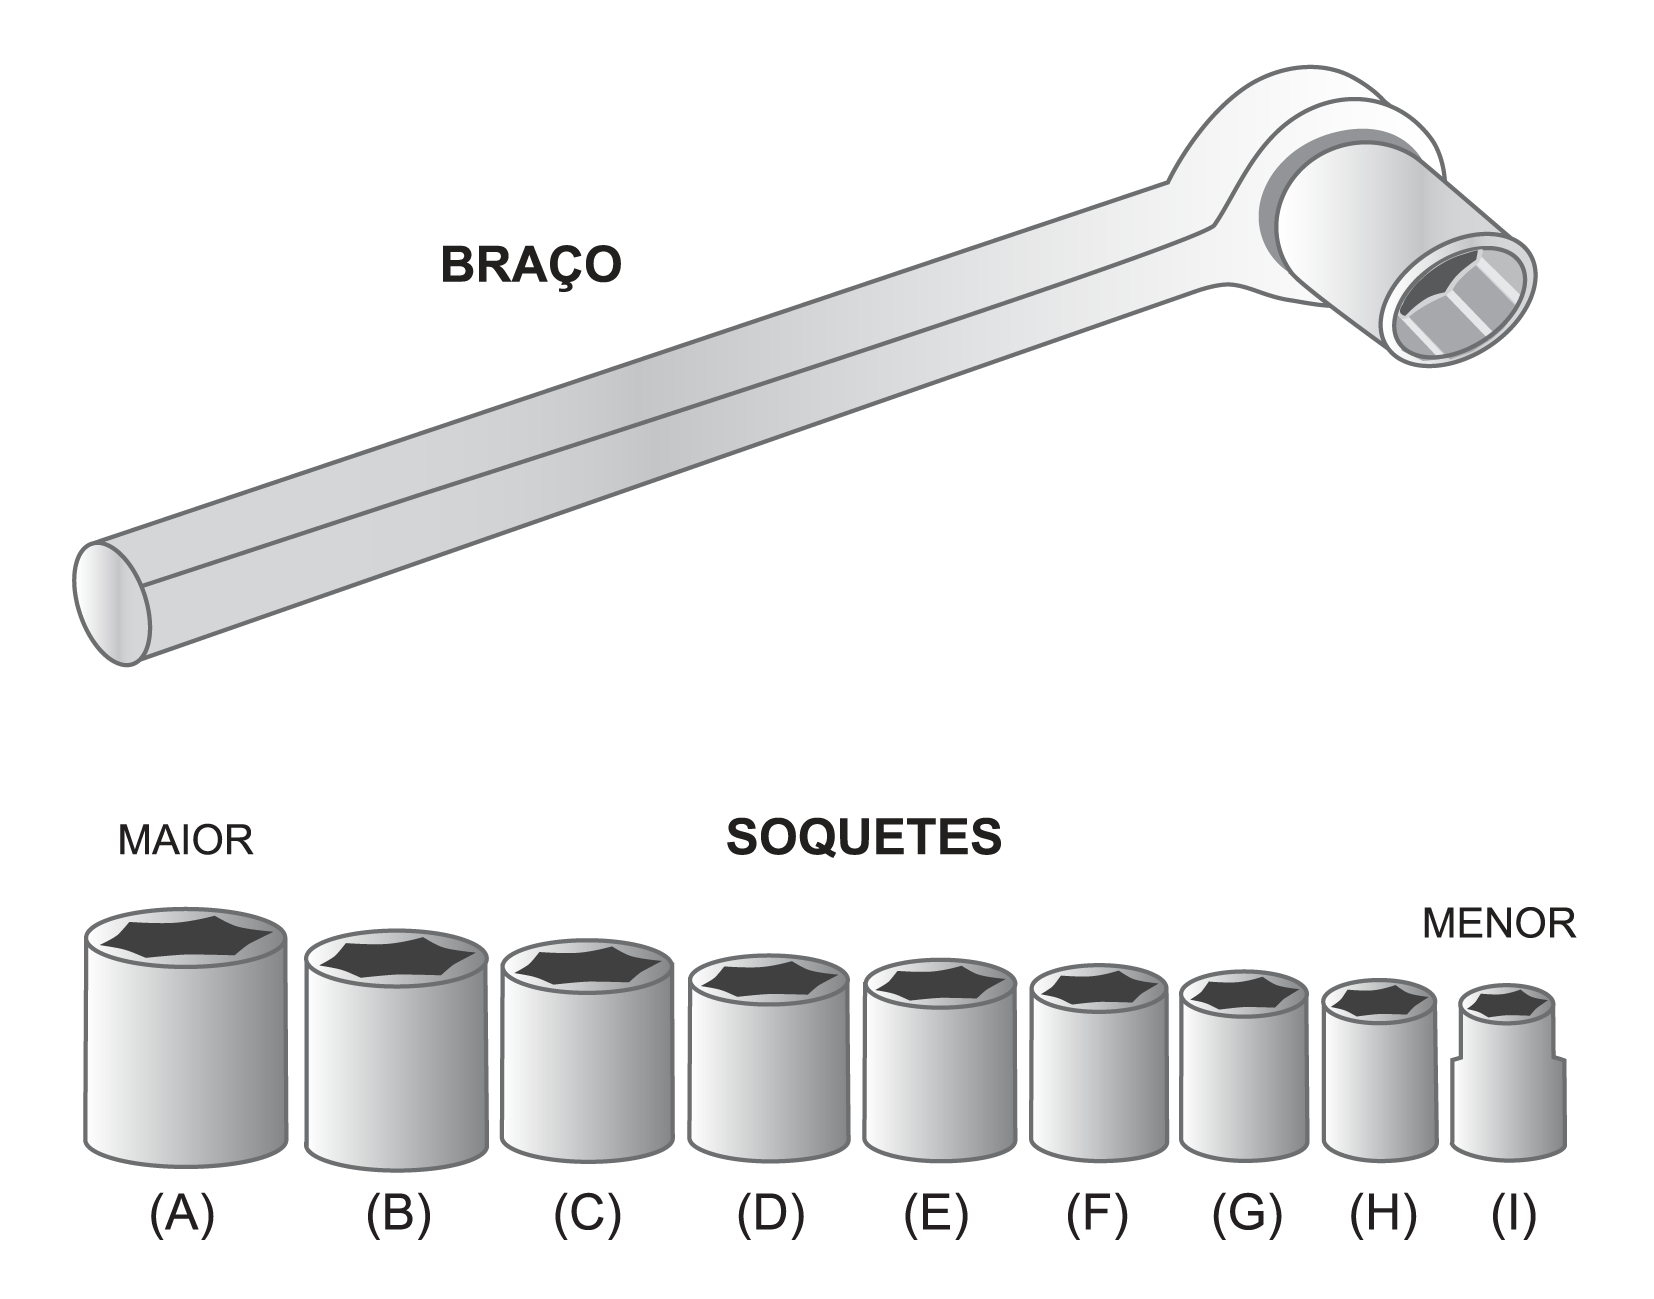
\includegraphics[width=300pt, keepaspectratio]{ativ14_fig01.png}
\end{center}

\ifdefined\prof
\begin{solucao}

Uma vez que   $\dfrac{1}{2} = \dfrac{8}{16}$  ,   $\dfrac{3}{4} = \dfrac{12}{16}$
,   $\dfrac{3}{8} = \dfrac{6}{16}$  ,   $\dfrac{5}{8} = \dfrac{10}{16}$   e
$\dfrac{7}{8} = \dfrac{14}{16}$  , os tamanhos dos soquetes são os seguintes:

(A):   $\dfrac{7}{8}$  ,
(B):   $\dfrac{13}{16}$  ,
(C):   $\dfrac{3}{4}$  ,
(D):   $\dfrac{11}{16}$  ,
(E):   $\dfrac{5}{8}$  ,
(F):   $\dfrac{9}{16}$  ,
(G):   $\dfrac{1}{2}$  ,
(H):   $\dfrac{7}{16}$  ,
(I):   $\dfrac{3}{8}$.

\end{solucao}
\fi

\end{document}